\section{Methodik} \label{sec_03}
Durch die wenigen beteiligten Personen ist ein simplifiziertes Wasserfallmodell ausreichend, um das Projekt durchzuführen.

Nach einer Analyse der Anforderungen und der Konzeption, bei der verschiedene Technologien verglichen werden und die grobe Struktur des Projektes festgehalten wird, geschieht die Umsetzung und daraufhin die Evaluation. In der Evaluation werden Faktoren wie das Einhalten der Anforderungen und die Codequalität überprüft.

\subsection{Anforderungsanalyse}
Da es sich um ein Forschungsprojekt handelt, können wirtschaftliche Aspekte einer Anforderungsanalyse zunächst vernachlässigt werden. Die Struktur der Analyse wird sich auf die Arbeit von Pandey, Suman und Ramani \cite{pandey2010effective} und dem Figma Template\cite{figma-use-case-template} für Use-Cases berufen. Sie bieten eine klare Struktur zur Identifizierung und Beschreibung der verschiedenen Anwendungsfälle für das Forschungsprojekt zur automatisierten Pflanzenpflege. Die definierten Use Cases ermöglichen es, die Bedürfnisse und Ziele der potenziellen Nutzenden sowie die erforderlichen Funktionen des Systems genau zu erfassen.

\subsubsection{Funktionale Anforderungen}
\paragraph{Use Case 1: Automatische Bewässerung}
\begin{itemize}
    \item Kunde: Pflanzenneuling
    \item System: Automatische Wasserpumpe
    \item Ziele des Kunden: Automatisches Gießen für eine gesunde Pflanze, er spart Zeit und muss sich keine Gedanken machen müssen
    \item Trigger: Neue Pflanze
\end{itemize}

Basic Flow:
Der Kunde erhält eine neue Pflanze. Er weiß den Namen, hat aber sonst keine weiteren Informationen. Er schließt die Pflanze, an das System an. Es wird automatisch die Bodenfeuchtigkeit ausgemessen und auf einem geeigneten Level gehalten.

Alternate Flow:
Der Kunde kennt bereits die gewünschte Bodenfeuchtigkeit. Das System nimmt diese auf und hält die Erde auf diesem Level.

\paragraph{Use Case 2: Überwachung der Pflanze}
\begin{itemize}
    \item Kunde: Interessierter Gärtner
    \item System: Automatische Sensoren
    \item Ziele des Kunden: Detaillierte Informationen über seine Pflanze, um diese besser zu pflegen
    \item Trigger: Neue oder ungesunde Pflanze, reines Interesse
\end{itemize}

Basic Flow:
Der Kunde schließt eine Pflanze an das System an. Das System misst regelmäßig alle nötigen Daten und gibt diese auf Anfrage aus. Der Kunde kann verschiedene Anfragen wie letzter Wert, Durchschnitte oder generelle Informationen über die Pflanze, Sonneneinstrahlung, Luftfeuchtigkeit, Bodenfeuchtigkeit und Temperatur, im Vergleich zum Optimum abfragen. Auch soll es mithilfe von Bildern Pflanzenwachstum über die letzten Wochen ausgeben können.

\paragraph{Use Case 3: Optimieren}
\begin{itemize}
    \item Kunde: Ergebnisorientierter Gärtner
    \item System: Automatische Sensoren und Wasserpumpe
    \item Ziele des Kunden: Die Pflanze soll möglichst schnell wachsen und blühen oder Früchte tragen.
    \item Trigger: Nicht optimale Werte der Pflanze bremsen das Wachstum aus.
\end{itemize}

Basic Flow:
Das System erkennt, dass bereitsfestgelegte Werte wie gewünschte Sonneneinstrahlung nicht optimal sind, da die Pflanze langsamer als gewöhnlich wächst. Es gibt Tipps um die Umweltsituation der Pflanze zu verändern und variiert die Frequenz des Gießens. Die neuen Daten werden verwendet, um weitere genauere Verbesserungsmöglichkeiten zu erkennen.

\subsubsection{Nicht-funktionale Anforderungen}
Die Anforderungen, die sich aus dem Konzept des Projekts, der technischen Umsetzung und verschiedenen Erfahrungen ergeben, bilden eine solide Grundlage für die Entwicklung des Systems zur automatisierten Pflanzenpflege. Im Folgendenden finden sich die nicht-funktionalen Anforderungen zusammengefasst:

\begin{itemize}
    \item Sprachgesteuerte Funktion: Das System soll vollständig durch Sprachbefehle gesteuert werden können, um eine intuitive Benutzererfahrung zu bieten.
    \item Reaktionszeit: Die Abfragen sollen in unter drei Sekunden geschehen, um dem Nutzer ein reibungsloses Erlebnis zu bieten. Anders als für Webseiten gibt es keine Studien, wie lange Nutzende gewillt sind bei einem Sprachassistenten auf eine Antwort zu warten. Aus Erfahrung mit verschiedenen Apps, sind drei Sekunden eine annehmbare Zeit für eine Reaktion.
    \item Regelmäßige Überprüfung des Pflanzenzustands: Das System soll den Zustand der Pflanze alle fünf Minuten überprüfen, um potenzielle Probleme schnell zu erkennen und zu korrigieren.
    \item Echtzeit-Datenerfassung und -speicherung: Das System soll jede Minute Werte der Pflanze erhalten und speichern, um Messfehler auszugleichen und zuverlässige Daten für Entscheidungen bereitzustellen.
    \item 24/7 Verfügbarkeit: Das System soll dem Benutzer jederzeit zur Verfügung stehen, um eine kontinuierliche Überwachung und Pflege der Pflanze zu gewährleisten.
    \item Automatische Geräteverbindung: Ein neues Gerät soll sich automatisch mit allen Diensten verbinden, ohne dass der Benutzer zusätzliche Eingaben vornehmen muss.
    \item Maximaler Ausfallzeitraum: Ein einzelnes Gerät darf (bei bestehender Internetverbindung und Stromzufuhr) maximal fünf Minuten ausfallen. So soll verhindert werden, dass über längere Zeit die Pflanze in nicht-optimalen Bedingungen wächst.
\end{itemize}

Später soll das System soll einmal die Woche Tipps zur Verbesserung der Umweltsituation geben. Die schnellsten Pflanzen zeigen jede Woche sichtbares Wachstum.\cite{sillplantgrowth} Ein späterer Machine Learning Ansatz kann so in sinnvollen Intervallen Änderungen zum Pflanzenwachstum geben und die Ergebnisse auswerten. 

\subsection{Grobkonzept}

\begin{figure}[H]
\centering
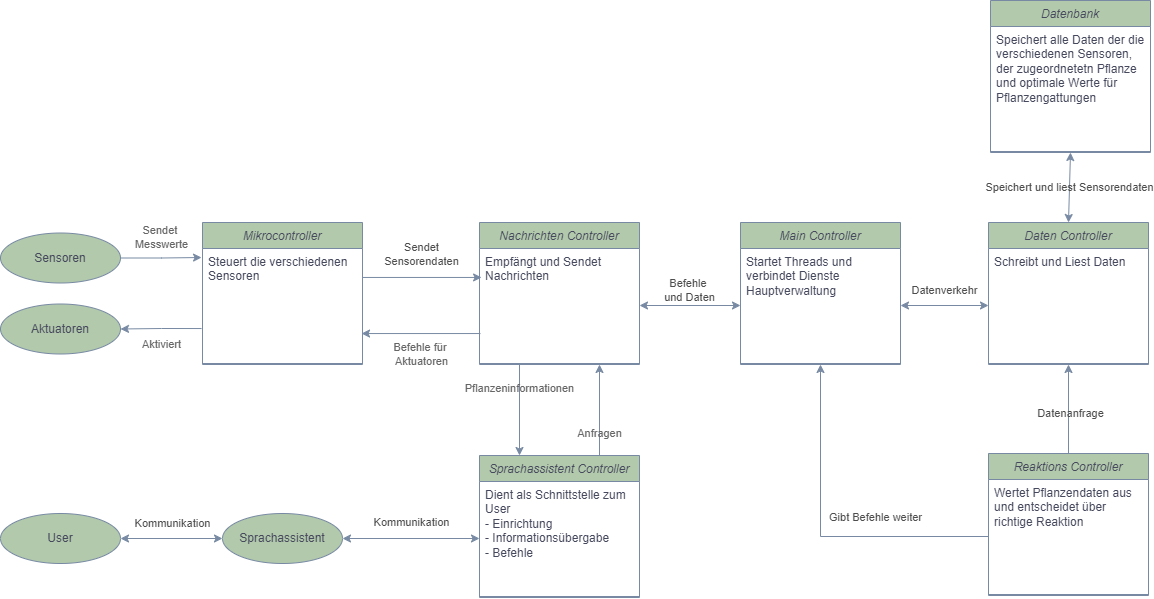
\includegraphics[width=\textwidth]{images/Grobkonzept_Flow.png}
\caption{Flowchart der allgemeinen Software-Architektur}\cite{rainpoint_smart_timer}
\label{fig:grob_flow}
\end{figure}

Das Grobkonzept der Architektur sieht neun verschiedene Teile vor. 

\begin{itemize}
    \item Sensoren
    \item Mikrocontroller
    \item Main Controller
    \item Nachrichten Controller
    \item Daten Controller
    \item Datenbank
    \item Reaktions Controller
    \item Sprachassistent Controller
    \item Sprachassistent
\end{itemize}

An einem Mikrocontroller sind verschiedene Sensoren und Aktuatoren angeschlossen. In regelmäßigem Abstand sammeln diese Umweltdaten und geben diese an den Controller weiter. Bei Bedarf kann dieser die Aktuatoren aktivieren. 
Drahtlos sendet der Mikroconroller die Daten an den Nachrichten Controller weiter. Dieser sendet diese an den Daten Controller, welcher sie in die Datenbank schreibt. 
In regelmäßigen Abständen holt der Main Controller über den Daten Controller die letzten Daten ein und gibt diese an den Reaktions Controller weiter. Dieser entscheidet, ob die Umweltdaten von den optimalen Werten abweichen. Ist dies der Fall wird der Befehl an den Mikrocontroller oder den Sprachassistenten weitergegeben. 
Der Nutzende interagiert mit der Maschine ausschließlich über einen Sprachassistenten. Über diesen können Anfragen gestellt werden, und diese teilt dem Nutzer automatisch wichtige Informationen zum Zustand der Pflanze zu oder empfiehlt eine Änderung des Umfelds.

Als Sensoren benötigen wir zunächst Messapparate für Licht, Temperature, Boden- und Luftfeuchtigkeit. Als Aktuatoren momentan lediglich eine Pumpe. Die Auswahl der Sensoren beruft sich auf die wichtigsten Umgebungsfaktoren für eine Pflanze.\cite{oregonenvironmentfactors}

\begin{figure}[H]
\centering
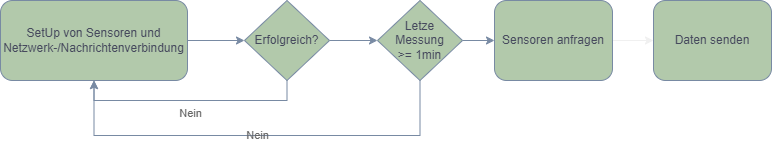
\includegraphics[width=\textwidth]{images/Grobkonzept_MikroCont.png}
\caption{Flowchart des Mikrocontrollers}\cite{rainpoint_smart_timer}
\label{fig:rainpointDiagram}
\end{figure}

Der Mikrocontroller soll jede Minute die Daten einohlen. 
Um die Funktionstüchtigkeit zu garantieren wird vor jeder Messung die Verbindung zu den Sensoren, der Netzwerkverbindung und dem Nachrichtendienst getestet. 
Funktioniert alles werden die Daten an den Nachrichten Controller gesendet. Erhält dieser diese speichert er sie in die Datenbank.

\begin{figure}[H]
\centering
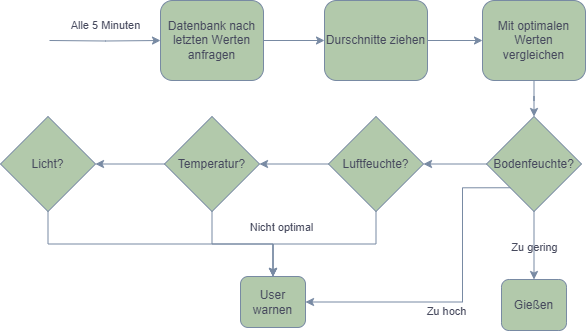
\includegraphics[width=\textwidth]{images/Grobkonzept_DatenCont.png}
\caption{Flowchart des Main Controllers}\cite{rainpoint_smart_timer}
\label{fig:rainpointDiagram}
\end{figure}

Alle fünf Minuten überprüft der Reaktions Controller, ob die gesendeten Daten mit den optimalen Werten für diese Pflanze übereinstimmen. 
Ist dies nicht der Fall wird der Nutzende darauf hingewiesen oder die Pumpe aktiviert.

\subsection{Feinkonzept}

\subsubsection{Auswahl des Mikrocontrollers}
Für die vorliegende Arbeit wurden spezifische Anforderungen identifiziert, die für das erfolgreiche Gelingen des Projekts von entscheidender Bedeutung sind. Zunächst ist eine zuverlässige Internetverbindung von höchster Priorität. Diese soll es ermöglichen, eine direkte Kommunikation mit dem Nachrichten Controller herzustellen, und so variabel für eine breite Palette von Anwendungsmöglichkeiten zu sein.

Des Weiteren war die Kompatibilität mit etablierten Bibliotheken ein wesentlicher Aspekt. Da verschiedene Sensoren benötigt werden, erleichtert die Verfügbarkeit einer Vielzahl von Bibliotheken die Entwicklung erheblich und ermöglicht ein einfache Softwaregestaltung, ohne aufwendige Workarounds.

Ein weiterer entscheidender Faktor war die Anzahl und Vielfalt der Anschlüsse. Um den Anforderungen des Projekts gerecht zu werden, war es wichtig, über ausreichend digitale und analoge I/O-Pins sowie verschiedene Kommunikationsschnittstellen zu verfügen.

Im Hinblick auf diese Anforderungen erwies sich der Arduino UNO R4 WiFi als optimale Lösung für das Projekt.\cite{arduino-uno-r4-wifi} Durch die Integration des ESP32-S3 Moduls bietet er die Möglichkeit, eine stabile drahtlose Verbindung herzustellen und somit eine Vielzahl von drahtlosen Anwendungen zu realisieren.

Darüber hinaus bietet der UNO R4 WiFi eine breite Unterstützung für gängige Bibliotheken und eine aktive Entwicklergemeinschaft, was die Entwicklung und Implementierung von Funktionen erleichtert und beschleunigt.

Die umfangreiche Anzahl an digitalen und analogen I/O-Pins sowie die Vielfalt der Kommunikationsschnittstellen ermöglichen eine flexible Konfiguration und Erweiterung des Systems, um den Anforderungen des Projekts gerecht zu werden.

Insgesamt erfüllt der Arduino UNO R4 WiFi die definierten Anforderungen für das Projekt und stellt somit die ideale Plattform für die erfolgreiche Umsetzung der gestellten Aufgaben dar.

\subsubsection{Auswahl der Sensoren}
Im Folgenden werden die Anforderungen und die darauffolgende Auswahl der Sensoren getroffen. Zu einer zuverlässigen Arbeitsweise und einer einfachen Integrierung in die Arduino-Umgebung kommen für den Typ des Sensors spezielle Anforderungen hinzu.

\paragraph{Licht}
Für die Lichtintensitätserkennung in diesem Projekt war es entscheidend, einen Sensor zu verwenden, der in der Lage ist, zwischen verschiedenen Lichtverhältnissen zu unterscheiden. Der LIGHT Unit Sensor erfüllt diese Anforderung durch die Integration eines Fotowiderstands und eines einstellbaren 10K-Widerstands.\cite{m5stack-light-sensor}

\begin{figure}[H]
\centering
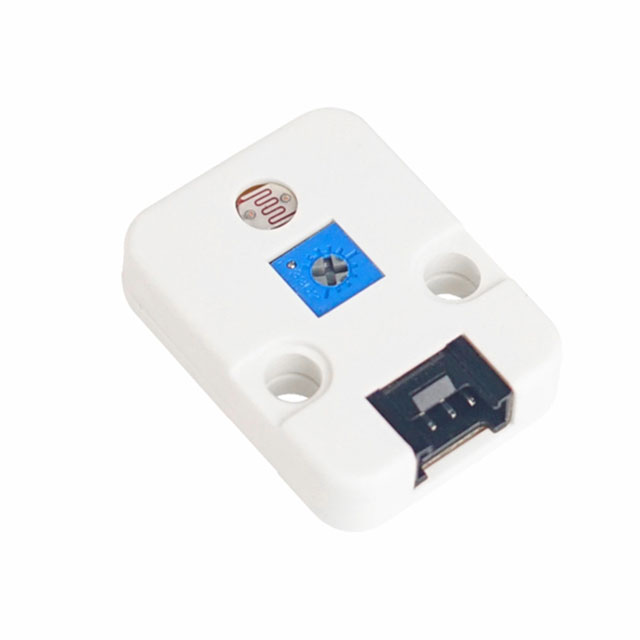
\includegraphics[width=0.5\textwidth]{images/LichtSensor.jpg}
\caption{Lichtsensor}\cite{rainpoint_smart_timer}
\label{fig:rainpointDiagram}
\end{figure}

Der Sensor ist in der Lage, die Lichtintensität zu erfassen und einen Schwellenwert für die Lichtintensität festzulegen. Dies ermöglicht die differenzierte Erkennung von Sonnenlicht. Durch die Erfassung der Spannungsänderung erhält der Sensor Lichtintensitätsdaten durch Analog-Digital-Umwandlung.

Um eine präzisere Lichtintensitätserkennung zu erreichen, integriert dieser Sensor auch einen LM393 Dual-Differenzverstärker. Dieser wird verwendet, um die differentielle Spannung zwischen dem Fotowiderstand und dem druckempfindlichen Widerstand zu vergleichen.

Die Kompatibilität mit verschiedenen Softwareentwicklungsplattformen wie Arduino erleichtert die Integration des Sensors in das Projekt und ermöglicht eine einfache Programmierung und Steuerung.

\paragraph{Temperatur und Luftfeuchtgkeit}
Für das Projekt war es von großer Bedeutung, genaue Werte für Temperatur und Luftfeuchtigkeit zu erhalten, ohne auf abstrakte Messungen angewiesen zu sein. Die Verwendung eines Sensors mit einer echten I2C-Schnittstelle war entscheidend, um eine einfache Integration in das Projekt zu ermöglichen und die Anforderungen an die Messgenauigkeit zu erfüllen.

Der Sensirion SHT40 Sensor erfüllt diese Anforderungen vollständig. Mit einer typischen relativen Feuchtigkeitsgenauigkeit von ±1,8 Prozent und einer typischen Temperaturgenauigkeit von ±0,2°C liefert der Sensor zuverlässige Messwerte über einen breiten Bereich von Temperaturen und Luftfeuchtigkeiten. \cite{adafruit-sht40}

\begin{figure}[H]
\centering
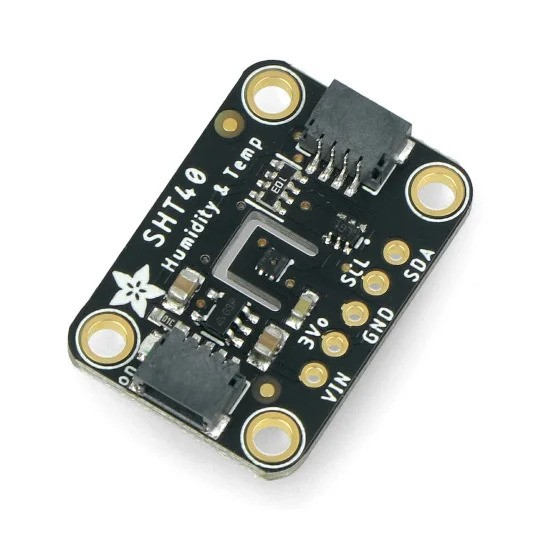
\includegraphics[width=0.5\textwidth]{images/TempSensor.jpg}
\caption{Temperatur- und Luftfeuchtigkeitssensor}\cite{rainpoint_smart_timer}
\label{fig:rainpointDiagram}
\end{figure}

Durch seine I2C-Schnittstelle ermöglicht der Sensor eine einfache Kommunikation mit anderen Geräten und Mikrocontrollern. Die Unterstützung des Sensors durch Arduino erleichtert die Programmierung und Integration in verschiedene Projekte und Plattformen. Zusätzlich bietet das Breakout-Board des Sensors eine einfache Handhabung und Integration in das Projekt, einschließlich SparkFun Qwiic-kompatibler STEMMA QT-Anschlüsse für den I2C-Bus.

\paragraph{Bodenfeuchtigkeit und Pumpe}
Die Watering Unit von M5Stack konnte die Feuchtigkeitsmessung durch Sensoren und eine Pumpe in einem Gerät vereinen. \cite{m5stack-watering-unit}

\begin{figure}[H]
\centering
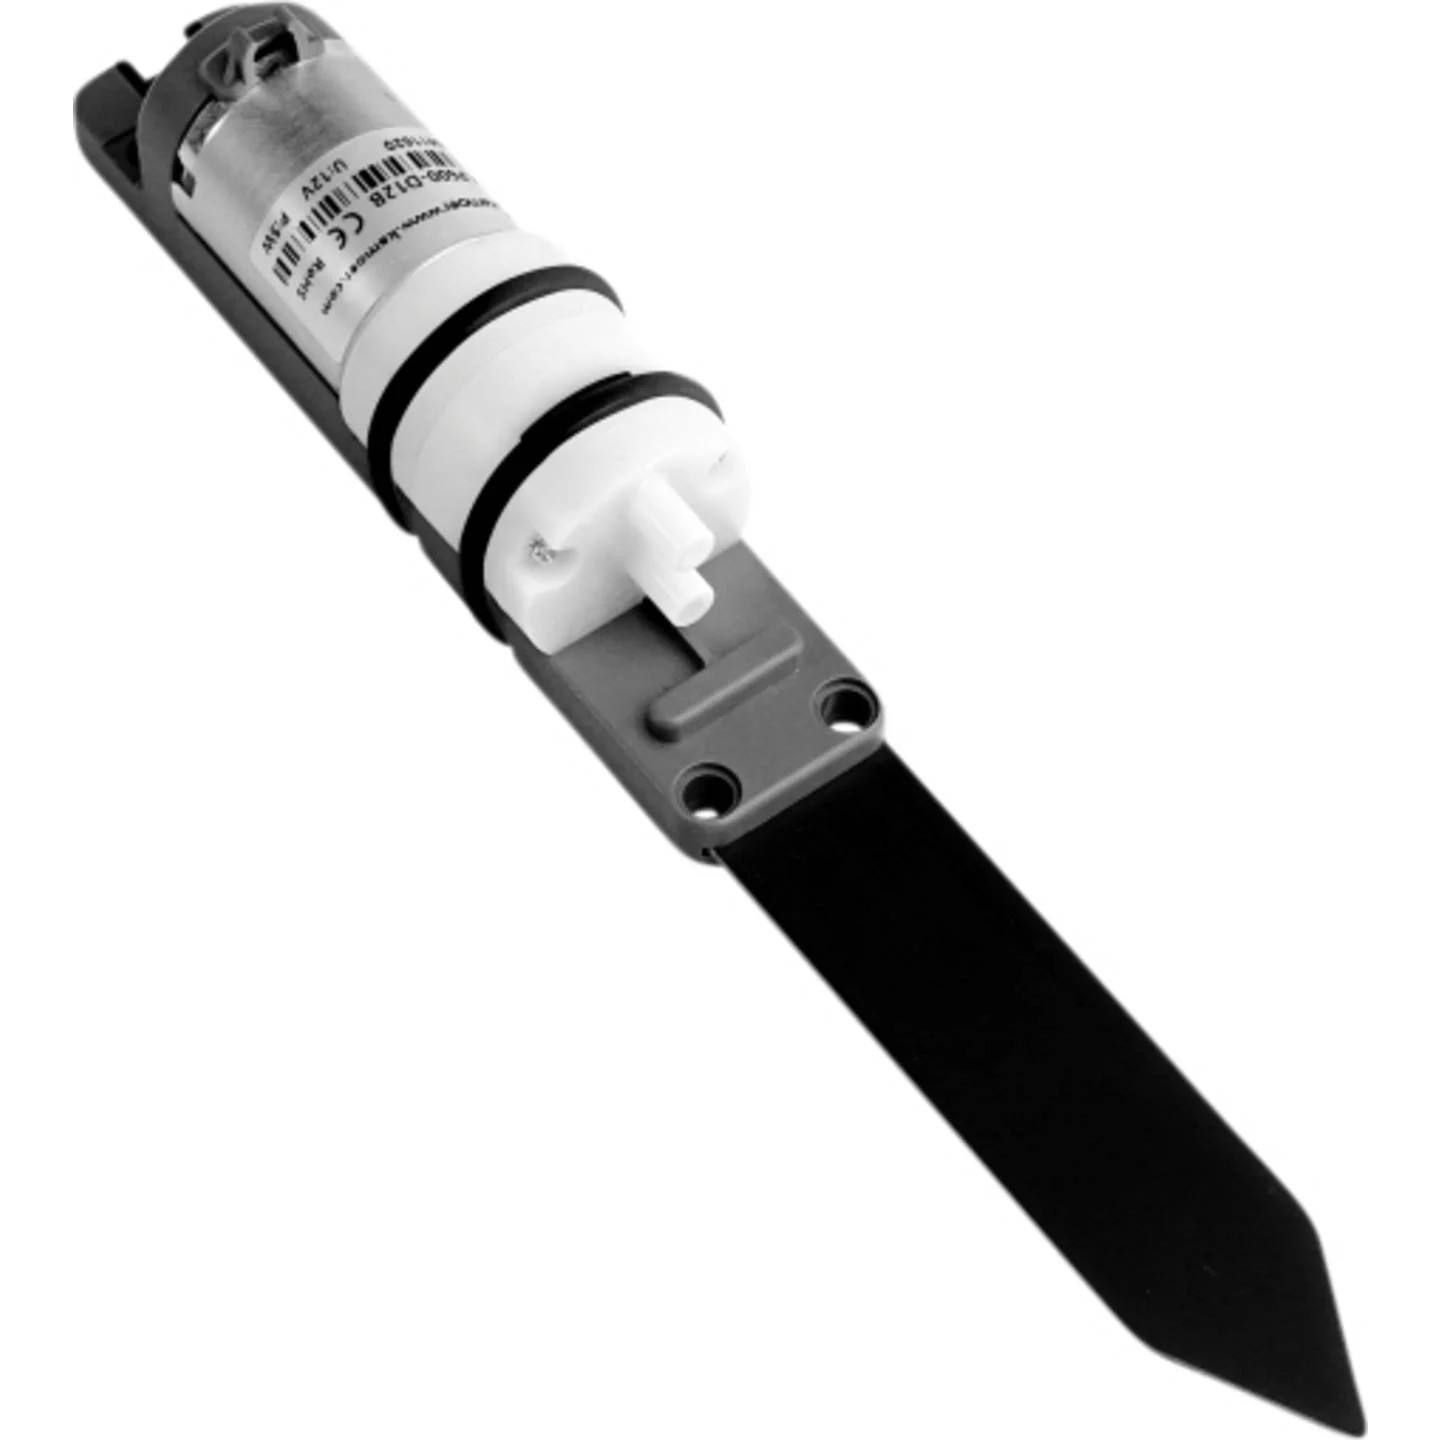
\includegraphics[width=0.5\textwidth]{images/Pumpe.jpg}
\caption{Pumpe und Bodenfeuchtigkeitssensor}\cite{rainpoint_smart_timer}
\label{fig:rainpointDiagram}
\end{figure}

Die Wassereinheit nutzt die Kapazitätsmessungstechnologie für die Bodenfeuchteerkennung. Die Sensorplatten sind kapazitiv gestaltet, was im Vergleich zu anderen Methoden eine höhere Korrosionsbeständigkeit bietet. Dadurch wird die Langzeitgenauigkeit der Feuchtigkeitsmessung gewährleistet.

Mit der integrierten Wasserumwälzpumpe kann die Einheit automatisch die Bewässerung basierend auf den gemessenen Bodenfeuchtigkeitswerten steuern. 

\paragraph{Kamera}
Für das Projekt ist es wichtig, eine Kamera zu finden, die ausreichend gute Bilder liefert, ohne außergewöhnliche Bildqualität zu erfordern. Da die Kamera statisch installiert ist, immer dieselbe Pflanze überwacht und lediglich die Maße des Objektes erkennen soll, nicht einzelne Zweige oder Farben, sind hohe Anforderungen an die Bildqualität nicht notwendig.

Die AZ Delivery Kamera erfüllt diese Anforderungen.\cite{azdelivery2024camera} Mit einer Auflösung von 640 x 480 Pixeln liefert sie ausreichend scharfe Bilder für die Projektanforderungen. Mit einer Größe von 3,5 cm Seitenlänge und 3 cm Höhe lässt sie sich einfach an der Pflanze platzieren.

\begin{figure}[H]
\centering
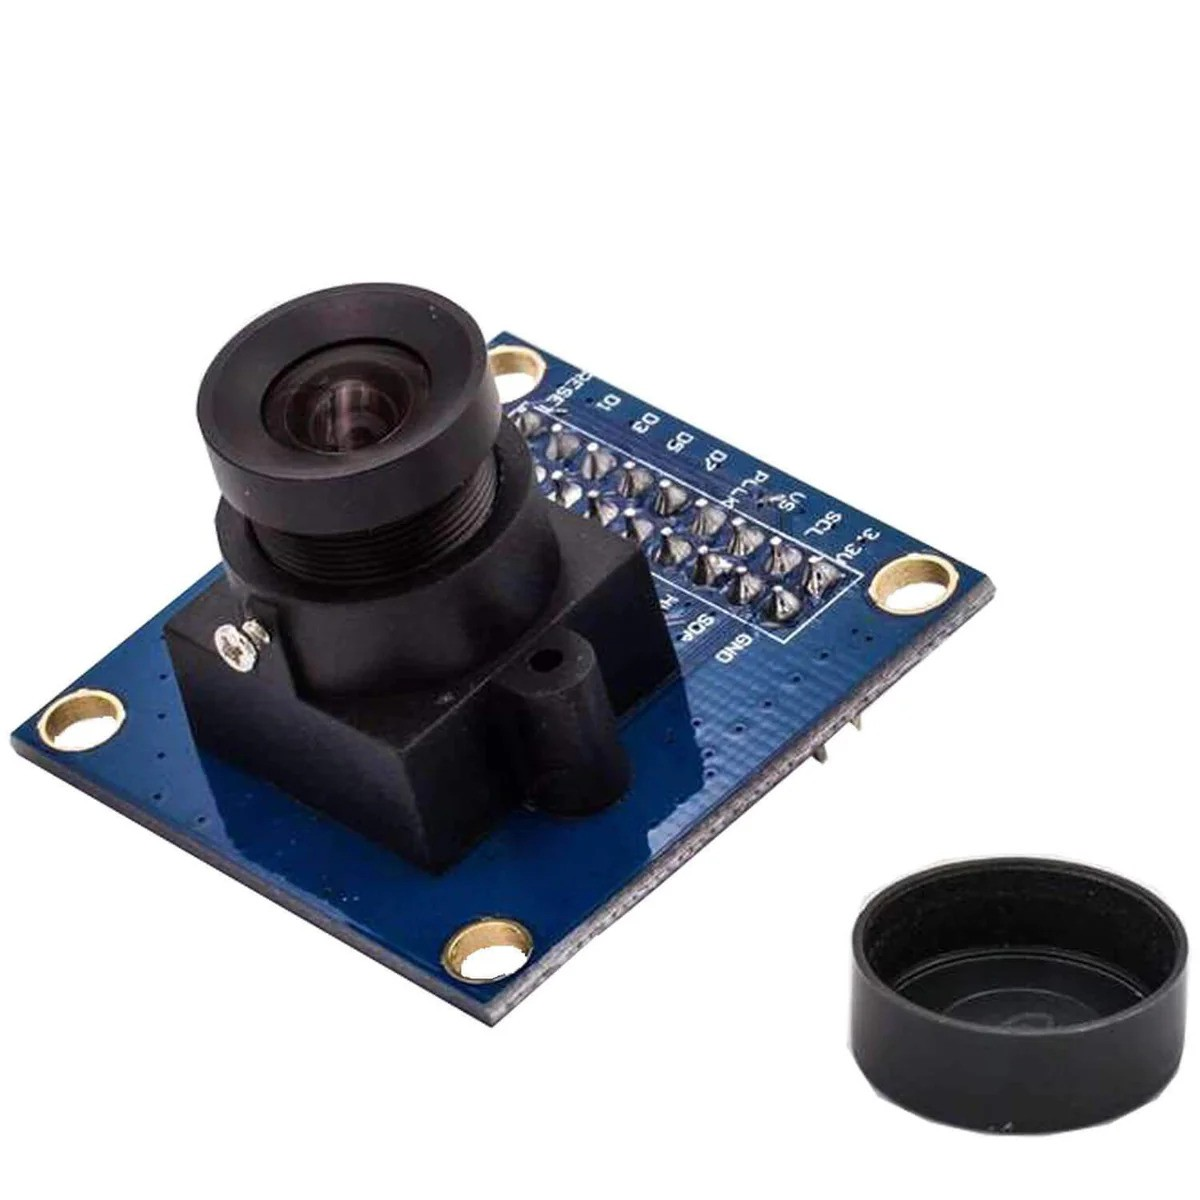
\includegraphics[width=0.5\textwidth]{images/Kamera.jpg}
\caption{Kamera}\cite{rainpoint_smart_timer}
\label{fig:rainpointDiagram}
\end{figure}

Der CMOS-Bildsensor bietet die volle Funktionalität einer VGA-Kamera und eines Bildprozessors in einem kompakten Gehäuse. Die Kamera ist mit Arduino kompatibel und kann Bilder in verschiedenen Formaten liefern, die über die Serial Camera Control Bus (SCCB)-Schnittstelle gesteuert werden. Sie kann mit bis zu 30 Bildern pro Sekunde in VGA-Auflösung aufnehmen, wobei der Benutzer die volle Kontrolle über die Bildqualität, das Format und die Datenübertragung hat.

\subsubsection{Nachrichtenprotokoll}
Für das Nachrichtenprotokoll zwischen dem Controller und dem Arduino war es wichtig, einen Nachrichtendienst zu wählen, der einfach zu handhaben ist, gut auf Ausfälle reagiert und stabil ist. Hierbei standen unter anderem MQTT, HTTP/REST und CoAP zur Auswahl.

MQTT ist der de-facto Standart für Iot-Projekte. Ausschlaggebend sind hierbei folgende Gründe: \cite{emqx2023mqtt}
\begin{itemize}
    \item Einfachheit: MQTT ist ein leichtgewichtiges Protokoll, das speziell für den Einsatz in eingeschränkten Umgebungen entwickelt wurde. Es ist einfach zu implementieren und erfordert minimale Bandbreite
    \item Robustheit: MQTT bietet eingebaute Mechanismen zur Erkennung und Behandlung von Verbindungsabbrüchen. Dies stellt sicher, dass Nachrichten zuverlässig zugestellt werden und die Kommunikation stabil bleibt. Ist ein Empfänger zur Zeit der Sendung nicht verfügbar bleibt das Netz trotzdem bestehen und die Nachricht wird gesendet.
    \item QoS (Quality of Service): MQTT bietet drei QoS-Stufen, die garantieren, dass Nachrichten je nach Bedarf mindestens einmal, höchstens einmal oder genau einmal zugestellt werden.
    \item Paketgröße: Durch die geringe Größe der MQTT-Pakete ist das Protokoll ideal für Geräte mit begrenzten Ressourcen und Netzwerkbandbreite.
\end{itemize}

HTTP (HyperText Transfer Protocol) ist das Standardprotokoll für die Kommunikation im Web. REST (Representational State Transfer) ist eine Architektur, die auf HTTP aufbaut und weit verbreitet für Webservices genutzt wird.

Es ist im Vergleich zu MQTT schwergewichtiger, da es mehr Overhead erzeugt. Es ist nicht so effizient in Bezug auf Bandbreitennutzung und Latenz. HTTP-Verbindungen sind auch weniger robust gegenüber Verbindungsabbrüchen, da sie keinen eingebauten Mechanismus zur Wiederverbindung haben.

CoAP ist ein spezialisiertes Webprotokoll für eingeschränkte Geräte und Netzwerke. Es basiert auf dem UDP-Protokoll und ist darauf ausgelegt, eine effiziente und schnelle Kommunikation zu ermöglichen. 

Es ist nicht so weit verbreitet wie MQTT und hat eine geringere Unterstützung in der Entwicklergemeinschaft. Ebenfalls ist es komplexer zu implementieren und zu warten, insbesondere in Bezug auf Sicherheitsaspekte.

Die Wahl fiel auf MQTT aufgrund seiner Einfachheit und Effizienz, die es ideal für IoT-Projekte macht. Es bietet robuste Mechanismen zur Handhabung von Verbindungsabbrüchen und sorgt für eine zuverlässige Kommunikation zwischen den Geräten. Im Vergleich zu HTTP/REST ist MQTT ressourcenschonender und besser für die Anforderungen eines IoT-Umfelds geeignet. CoAP wurde aufgrund seiner geringeren Verbreitung und höheren Komplexität verworfen, obwohl es in bestimmten Szenarien ebenfalls eine gute Wahl sein kann. MQTT bietet jedoch die beste Kombination aus Stabilität, Einfachheit und Effizienz für das vorliegende Projekt.

\subsubsection{Programmiersprache}
Arduino Projekte werden standardmäßg in C++ geschrieben. Um die nötigen Bibliotheken, wie MQTT oder spezifische Sensorenfunktionen zu benutzen, wurde von C++ nicht abgewichen.

Für die Implementierung der Controller wurde Python als Programmiersprache gewählt. Diese Entscheidung basierte auf den zahlreichen Vorteilen, die Python speziell für das Projekt bietet.\cite{javatpoint2021iotpython}

Ein wesentlicher Grund für die Wahl von Python ist die umfangreiche Verfügbarkeit von Bibliotheken und Frameworks. Python bietet eine Vielzahl von Bibliotheken, die speziell für IoT-Anwendungen entwickelt wurden, wie beispielsweise `paho-mqtt` für die MQTT-Kommunikation. Zudem existieren mehrere Web-Frameworks in Python, wie Flask oder Django für Web-Interfaces, falls diese in einer späteren Iteration des Projektes integriert werden sollten.

Ein weiterer Vorteil ist die einfache Implementierung. Die Sprache ist bekannt für ihre klare und leicht verständliche Syntax, die es Entwicklern ermöglicht, schnell funktionalen Code zu schreiben und zu verstehen. Diese einfache Syntax und die hohe Abstraktionsebene von Python ermöglichen einen schnellen Workflow und Entwicklung, was besonders in der dynamischen und iterativen Welt der IoT-Projekte von Vorteil ist.

Python bietet zudem weitreichenden Support für KI-Funktionen. Die Sprache ist die bevorzugte Wahl für maschinelles Lernen und künstliche Intelligenz, mit umfangreichen Bibliotheken wie TensorFlow, Keras und scikit-learn, die problemlos in das Projekt integriert werden können. Auch für die Datenanalyse ist Python hervorragend geeignet, mit Bibliotheken wie Pandas und NumPy, die eine effiziente Analyse und Verarbeitung großer Datenmengen ermöglichen.

Die große und aktive Community stellt einen weiteren Pluspunkt dar. Diese Gemeinschaft bietet umfangreiche Unterstützung, von Tutorials und Foren bis hin zu Open-Source-Projekten und Beispielcodes. Zudem wird Python kontinuierlich weiterentwickelt und regelmäßig aktualisiert, wodurch die Sprache stets aktuell bleibt und sich kontinuierlich verbessert.

Java hingegen ist eine weit verbreitete Programmiersprache und bietet ebenfalls Plattformunabhängigkeit und eine große Anzahl an Bibliotheken. Allerdings ist der Entwicklungsprozess in Java oft komplexer und zeitaufwändiger. Java erfordert oft ausführlichere Boilerplate-Codes. Dies kann die Entwicklungsgeschwindigkeit und die Flexibilität bei schnellen Iterationen, die für IoT-Projekte notwendig sind, beeinträchtigen.

C ist eine sehr leistungsfähige Sprache, die besonders in der Embedded-Entwicklung weit verbreitet ist. Sie bietet eine feingranulare Kontrolle über die Hardware und ist extrem effizient. Allerdings ist die Entwicklung in C im Vergleich zu Python deutlich komplizierter und fehleranfälliger. Die manuelle Speicherverwaltung und die weniger abstrahierte Syntax erhöhen die Komplexität und das Risiko von Fehlern. Zudem fehlen in C viele der modernen Bibliotheken und Frameworks, die Python für IoT und KI bietet.

Zusammenfassend bietet Python durch seine umfangreichen Bibliotheken, einfache Implementierung, Unterstützung für KI-Funktionen und starke Community eine ideale Grundlage für die Entwicklung von IoT-Projekten. Es ermöglicht eine schnelle Entwicklung und einfache Integration von Hardware- und Softwarekomponenten.

\subsubsection{Auswahl der Datenbank}

Generell gibt es viele verschiedene Arten von Datenbanken. Hierzu gehören dokumentenbasierte wie etwa MongoDB, relationale Datenbanken wie PostgreSQL oder graphische wie Neo4j. Aufgrund der Popularität von IoT-Projekten und der hohen Nachfrage exisitieren inzwsichen zahlreiche auf IoT spezialisierte Datenbanken, wie etwa InfluxDB, TimescaleDB, CrateDB oder RethinkDB. Diese sind speziell für die großen Datenmengen angefertigt, welche jedoch einzeln nicht viel Speicher einnehmen. Im Normalfall werden nur einzelne Zahlen mit einem Tag gespeichert. Diese Time-Series Datenbanken verknüpfen neue Informationen automatisch mit einem Zeitstempel.

Für die Speicherung von Daten wurde InfluxDB als Datenbank ausgewählt. \cite{influxdata2021iot} 

InfluxDB eignet sich aufgrund seiner Fähigkeit, einzelne Zahlenwerte mit genauen Zeitstempeln zu speichern, die leicht zu lesen und zu schreiben sind und schnelle Berechnungen ermöglichen. Dies ist besonders wichtig für die Anforderungen des Projekts, bei dem kontinuierlich Daten erfasst und analysiert werden müssen.

Ein wesentlicher Vorteil von InfluxDB liegt in seiner spezialisierten Auslegung für Daten. Im Gegensatz zu relationalen Datenbanken verwendet InfluxDB ein NoSQL-Modell, was das Schreiben von Daten erheblich beschleunigt. Komplexe Datenstrukturen sind nicht erforderlich, was die Effizienz erhöht. 

Ein weiterer Grund für die Wahl von InfluxDB ist die Möglichkeit, einen eigenen Server zu hosten. Dies bietet Flexibilität und Kontrolle über die Datenbankumgebung, ohne zusätzliche Kosten. InfluxDB bietet eine kostenfreie Lösung, die es ermöglicht, die Datenbankumgebung an spezifische Projektanforderungen anzupassen und sie skalierbar zu halten.

Ein weiterer technischer Vorteil ist die Leistungsfähigkeit von InfluxDB bei der Skalierung und Verarbeitung großer Datenmengen. InfluxDB kann massive Mengen an IoT-Telemetrie-Daten ingestieren und indizieren, während es gleichzeitig Echtzeitanalysen und schnelle Abfragezeiten bietet. Dies ist entscheidend, da die Menge der IoT-Daten und die Anforderungen an deren Verarbeitung schnell wachsen.

Die Nutzung der Flux-Abfragesprache von InfluxDB ermöglicht es, Daten sowohl zu formen als auch abzufragen, was die Komplexität reduziert und die Effizienz erhöht. Flux bietet leistungsstarke Funktionen zur Datenanalyse direkt auf der Datenbankebene, ohne dass teure Abfragen zum Herunterladen und Modifizieren der Daten erforderlich sind.

Zusammenfassend bietet InfluxDB durch seine spezialisierten Funktionen für Zeitreihendaten, die schnelle und einfache Datenverarbeitung und die Fähigkeit zur Skalierung eine ideale Lösung für die Anforderungen des Projektes.

\subsubsection{Sprachsteuerung}
Für die Sprachsteuerung des IoT-Projektes wurde Alexa ausgewählt. Alexa ist der führende Anbieter von Smart-Speaker.\cite{fleck2024smartspeakers} Außerdem ermöglicht es mit dem Alexa Skills Kit (ASK) die Erstellung eigener Programme, sogenannte Skills. Es ist hiermit um einiges offener als vergleichbare Sprachassistenten, wie etwa Google Home.Diese Skills sind Anwendungen, die eine interaktive Sprachschnittstelle verwenden, um Nutzern verschiedene Interaktionen zu ermöglichen. Nutzer können Alexa Skills verwenden, um alltägliche Aufgaben zu erledigen, wie zum Beispiel Nachrichten abzurufen, Musik zu hören oder Spiele zu spielen. Zudem können Nutzer ihre Stimme nutzen, um cloud-verbundene Geräte zu steuern, wie beispielsweise das Einschalten von Lichtern oder das Anpassen des Thermostats.

Die Auswahl für Alexa beruft sich auf verschiedene Vorteile: \cite{amazon2024alexa}
\begin{itemize}
    \item Alexa ist weit verbreitet und wird in zahlreichen Haushalten genutzt. Dies erhöht die Akzeptanz und die Nutzerfreundlichkeit, da viele Nutzer bereits mit der Funktionsweise von Alexa vertraut sind.
    \item Die einfache Verbindung von Alexa mit Amazon Web Services (AWS) ist ein entscheidender Vorteil. AWS bietet eine robuste Infrastruktur, die die Skalierbarkeit und Zuverlässigkeit des Projekts sicherstellt. Zudem ermöglicht die Nutzung von AWS Lambda eine effiziente und kostengünstige Serververwaltung, da keine eigenen Server erforderlich sind.
    \item ASK bietet eine umfassende Entwicklungsumgebung, die APIs, Tools, Code-Beispiele und technische Dokumentation umfasst. Dies erleichtert die Erstellung und Verwaltung von Skills erheblich. Insbesondere die Nutzung des Alexa-Developer-Consoles und der ASK SDKs in Programmiersprachen wie Node.js, Java und Python vereinfacht den Entwicklungsprozess. 
\end{itemize}

Nutzer greifen auf Skill-Inhalte zu, indem sie Alexa auffordern, den Skill zu aktivieren. Nachdem das Aktivierungswort "Alexa" gesagt wird, verarbeitet der Alexa-Dienst die Sprachdaten in der Cloud. Alexa erkennt die Sprache, bestimmt die Intention des Nutzers und sendet eine Anfrage zur Ausführung des entsprechenden Skills. Der Skill läuft als Dienst auf einer Cloud-Plattform und kommuniziert über eine HTTPS-Schnittstelle mit Alexa. Bei Aktivierung eines Alexa-Skills erhält der Skill eine POST-Anfrage mit einem JSON-Body, der die notwendigen Parameter zur Verarbeitung und Beantwortung der Anfrage enthält.

Alexa Skills nutzen Sprachinteraktionsmodelle, um festzulegen, welche Worte und Phrasen Nutzer sagen können, um den Skill zu steuern. Es gibt zwei Haupttypen von Sprachinteraktionsmodellen:

\begin{itemize}
    \item Vorgefertigt: ASK definiert die zu verwendenden Worte und Phrasen. Zum Beispiel: "Alexa, schalte das Licht ein."
    \item Benutzerdefiniert: Dieses Modell bietet  Flexibilität und erfordert die Definition aller möglichen Arten, wie ein Nutzer eine Anfrage stellen könnte.
\end{itemize}

Der Entwurf eines Alexa Skills sollte natürlich, nutzerzentriert und visuell ansprechend sein. Die Entwicklung beginnt mit dem Design des Sprachinteraktionsmodells, gefolgt von der eigentlichen Implementierung des Skills. Die Verwendung des Alexa-Developer-Consoles oder Visual Studio Code ermöglicht das Testen des Skills während der Entwicklung.

ASK stellt Tools zum Testen des Skills zur Verfügung, darunter der Alexa-Simulator und die Alexa-App. Vor der Veröffentlichung muss der Skill den Zertifizierungsprozess durchlaufen, um sicherzustellen, dass er den Qualitäts-, Sicherheits- und Richtlinienanforderungen entspricht.

Nach der Veröffentlichung können Skills überwacht und analysiert werden. Die Entwicklerkonsole bietet Einblicke in die Nutzung, Analysen und Einnahmenverwaltung. Bei Problemen kann auf eine vorherige Version des Skills zurückgegriffen werden.

\subsubsection{Testing}
Zur Qualitätssicherung und Funktionsprüfung des IoT-Projektes wurden eine Mischung aus Cucumber-Tests und Unit-Tests eingesetzt. Diese Teststrategien ergänzen sich und bieten eine umfassende Abdeckung der Softwarequalität.

\paragraph{Cucumber-Testing}
Cucumber ist ein Werkzeug zur Verhaltensgesteuerten Entwicklung (Behavior-Driven Development, BDD). \cite{smartbear2019cucumber}Es ermöglicht die Erstellung von Tests in einer für Menschen lesbaren Sprache, meist in Gherkin-Syntax, die sowohl von Entwicklern als auch von Fachexperten verstanden wird. Ein typisches Cucumber-Szenario besteht aus drei Teilen:

\begin{itemize}
    \item Given: Definiert den Anfangszustand
    \item When: Beschreibt die Aktion oder das Ereignis.
    \item Then: Beschreibt das erwartete Ergebnis.
\end{itemize}

Cucumber-Tests werden verwendet, um ganze Funktionen oder Anwendungsfälle zu testen. Sie helfen dabei, die Anforderungen des Geschäftsbereichs direkt mit den Entwicklungsergebnissen zu verknüpfen, indem sie sicherstellen, dass die entwickelten Funktionen den definierten Geschäftsregeln und -anforderungen entsprechen. Sie schaffen eine gemeinsame Sprache für die Beschreibung der Anforderungen und reduzieren so Missverständnisse

\paragraph{Unit-Testing}
Unit-Tests sind eine Form der Softwaretests, die einzelne Komponenten oder Einheiten des Quellcodes isoliert überprüfen. Diese Tests fokussieren sich auf kleine Codeabschnitte, wie Funktionen oder Methoden, und prüfen deren Korrektheit unabhängig vom Rest des Systems. Unit-Tests werden oft automatisiert und bieten schnelle Rückmeldung über den Zustand des Codes.

Unit-Tests werden verwendet, um kleine Codeeinheiten detailliert zu prüfen. Sie ermöglichen es, Fehler frühzeitig im Entwicklungsprozess zu erkennen und zu beheben, und tragen so zur Stabilität und Zuverlässigkeit des Codes bei.

\paragraph{}
Eine Kombination der beiden Testarten führt zu einer umfassenden Testabdeckung auf unterschiedlichen Abstraktionsebenen. Während Cucumber-Tests sicherstellen, dass die Software den Geschäftsanforderungen entspricht, garantieren Unit-Tests die technische Integrität der einzelnen Codeeinheiten. Zusätzlich verbessern sie die Wartbarkeit und Weiterentwicklung der Software. Cucumber-Tests dienen als lebende Dokumentation der Geschäftslogik, während Unit-Tests die technische Basis absichern. Dies erleichtert zukünftige Änderungen und Erweiterungen, da sowohl die Geschäftslogik als auch die Codeintegrität kontinuierlich geprüft werden.

\subsubsection{Deployment Verfahren}
Docker wurde für das Projekt ausgewählt, um eine effiziente Bereitstellung und Verwaltung der IoT-Anwendung zu gewährleisten. Die Hauptgründe für die Wahl von Docker sind wie folgt:

\begin{itemize}
    \item Effizientes Herunterladen und Bereitstellen: Docker ermöglicht es, Anwendungen in Container zu verpacken, die alle erforderlichen Abhängigkeiten enthalten. Dadurch kann die Anwendung auf verschiedenen Rechnern identisch und effizient bereitgestellt werden. Das Herunterladen eines Docker-Images ist oft schneller und weniger fehleranfällig als das Einrichten einer Entwicklungsumgebung von Grund auf.
    \item Plattformunabhängigkeit: Mit Docker ist sichergestellt, dass die Anwendung in jeder Umgebung gleich läuft, sei es auf einem lokalen Rechner, einem Server oder in der Cloud. Dies reduziert die Probleme, die durch unterschiedliche Systemkonfigurationen entstehen können.
    \item Versionenkontrolle: Docker-Images können versioniert werden, was es ermöglicht, jederzeit zu einer vorherigen Version zurückzukehren. Dies ist besonders wichtig für die Nachverfolgbarkeit von Änderungen und die Sicherstellung der Stabilität der Anwendung.
    \item Einbindung von Tests: Docker unterstützt die Integration von automatisierten Tests, indem Testumgebungen schnell und konsistent bereitgestellt werden können. Dies fördert eine kontinuierliche Integration und kontinuierliches Testen (CI/CD), was die Qualität und Zuverlässigkeit der Anwendung erhöht.
\end{itemize}

Durch die Verwendung von Docker konnte die IoT-Anwendung effizient, konsistent und zuverlässig bereitgestellt und verwaltet werden, was zu einer verbesserten Entwicklungs- und Betriebsumgebung führte.

\subsubsection{Serverinfrastruktur}
Für das Projekt wurde ein Universitätsserver genutzt, der den Anforderungen entsprechend kostenfrei zur Verfügung gestellt wurde und alle notwendigen Richtlinien erfüllte. Der E-Mail-Verkehr mit dem Administrator Holger Szüsz verdeutlicht die wesentlichen Aspekte der Servernutzung und deren Infrastruktur.

\paragraph{Anforderungen}
Kontinuierlicher Betrieb, um eine ununterbrochene Datenerfassung zu gewährleisten.
Geringe Rechenleistung und Speicherplatz: Die Anwendung benötigt pro Stunde etwa 157 MB Speicher und verursacht einen minimalen I/O-Datenverkehr von ca. 3 KB die Sekunde.
Docker-Infrastruktur: Es werden zwei unabhängig voneinander arbeitende Container benutzt, die Datenbank und der Controller.
Geringer Netzwerkverkehr: Nach einer Stunde beträgt der Netzwerkverkehr etwa 1.9 MB eingehend und 1.8 MB ausgehend.

\paragraph{Serverkapazität}
Der bereitgestellte Server, ist mit leistungsstarken Komponenten ausgestattet:
\begin{itemize}
    \item Prozessor: Intel i9, der für komplexe Berechnungen und Analysearbeiten geeignet ist.
    \item Grafikkarte: NVIDIA RTX 4090, die für grafikintensive Anwendungen und potenziell für maschinelles Lernen genutzt werden kann.
\end{itemize}
Mit diesen Ressourcen könnten auch spätere, aufwendige KI-Berechnungen durchgeführt werden.

\paragraph{}
Der Administrierende hat einen Benutzeraccount eingerichtet, der mit den gleichen Zugangsdaten wie das Lehr-Login genutzt werden kann. Der Zugriff auf den Server erfolgt über SSH, was auch ohne VPN möglich ist, falls Netzwerkprobleme auftreten.

Um den Zugriff zu erleichtern und die Sicherheit zu erhöhen, wurde empfohlen, SSH-Keys auf dem Login-Server zu hinterlegen, was die Authentifizierung vereinfacht und absichert.

\subsection{Theoretisches Konzept}
In diesem Teil wird die theoretische Vorgehensweise für die Bildauswertung und die Anpassung der Optimalwerte geschildert. Da eine Umsetzung den Rahmen der Arbeit übersteigt, werden lediglich Ansätze vorgestellt, um die dargelegten Problematiken zu lösen.

\paragraph{Bildauswertung}
Wie in vorangegangenen Projekten gezeigt wurde, ist Bildauswertung ein großes Feld, das je nach Anforderungen sehr komplex sein kann. Inzwischen gibt es jedoch verschiedene Bibliotheken, insbesondere in der Programmiersprache Python, die die Objekterfassung deutlich erleichtern. Da kleinere Messfehler in diesem Projekt der privaten Nutzung keine größeren Schäden verursachen und die Kamera stationär befestigt ist, ist es für einen ersten Prototypen ausreichend, Standardbibliotheken zu verwenden. Die folgende Methodik beruft sich größtenteils auf ein Projekt von Adrian Rosebrock.\cite{pyimagesearch2024measuring}

Generell muss bei einer Größeneinschätzung die Anzahl der Pixel in Relation zu einer Maßeinheit gebracht werden. Um das Modell zu trainieren, werden daher Bilder von verschiedenen Pflanzen benötigt, sowie ihre Maße (Höhe und Breite). Außerdem sollten die Objekte leicht zu identifizieren sein; ein einfarbiger Hintergrund vereinfacht daher das Training. Zudem sollte ein Referenzobjekt enthalten sein, beispielsweise ein Kreis auf dem Hintergrund, sodass das Objekt einfacher zu messen ist.

Anhand verschiedener Bilder können wir so die Relation des Objektes berechnen: Pixel geteilt durch wahre Länge. In diesem Fall werden die Berechnungen sowohl für die Pflanze als auch das Referenzobjekt durchgeführt. So können auch bei anderen Pflanzen zuverlässige Ergebnisse erzielt werden.

Um das Modell zu trainieren, sollten einzelne Bilder in Graustufen unterteilt werden. Mithilfe von OpenCV, einer Bibliothek für Bildverarbeitung und Computer-Vision, können Konturen erkannt und gekennzeichnet werden. Mithilfe dieser Konturen kann OpenCV einzelne Objekte identifizieren.\cite{opencv2023objectdetection}

\begin{figure}[H]
\centering
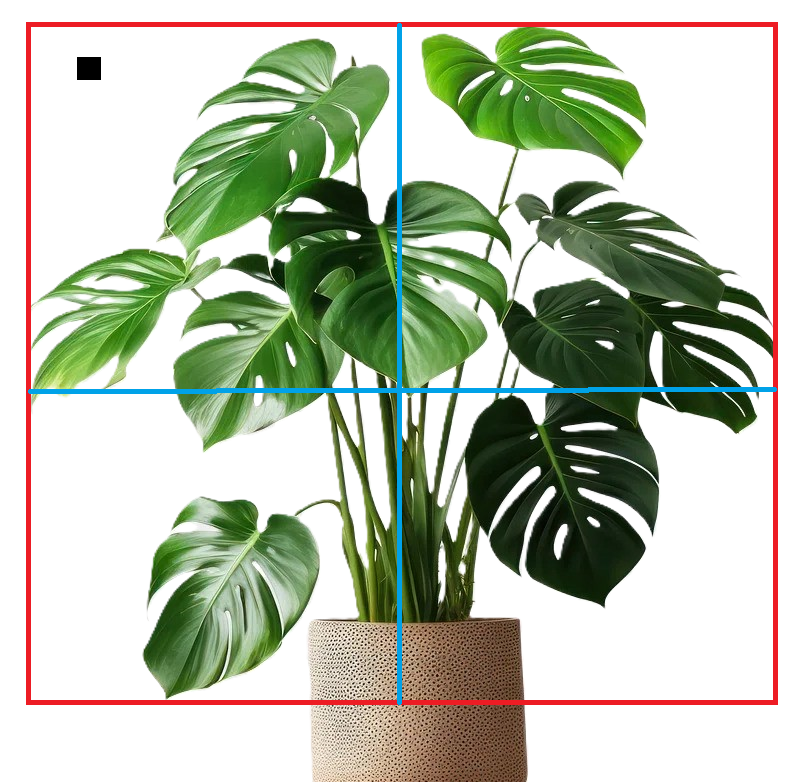
\includegraphics[width=0.8\textwidth]{images/massePlant.png}
\caption{Messung einer Pflanze mittels Object Detection}\cite{rainpoint_smart_timer}
\label{fig:rainpointDiagram}
\end{figure}

Sind die vier Seiten des Objektes eingegrenzt (rot), können Berechnungen durchgeführt werden, um die Maße zu bestimmen. Zunächst werden die Mittelpunkte der Seiten eingezeichnet, von diesen werden Linien zu den anderen Seitenmittelpunkten gezogen (blau), sodass  ein Kreuz in dem Objekt-Rechteck entsteht. Diese zwei Linien werden in Relation zu den realen Daten gesetzt. 
Im Beispiel ist die blaue horizontale Linie 755 Pixel lang, die vertikale 682 Pixel. In echt wurde die Pflanze auf etwa 20,5cm breit und 19cm hoch gemessen. Das Quadrat ist bei 0,5cm 18 Pixel groß.

Wird das Modell, mit verschiedenen Pflanzen in verschiedenen Wachstumsphasen, mit ausreichend Daten trainiert, kann es, mithilfe des Referenzobjektes, sinnvolle Ergebnisse erzielen.

Sollten die initalen Ergebnisse nicht ausreichen, können mit mehr und genaueren Daten, verschiedenen Bildern aus unterschiedlichen Perspektiven und mehr Pre-Processing mithilfe der OpenCV-Bibliothek, die Ergebnisse weiter verbessert werden.

\paragraph{Anpassung der Optimalwerte durch Machine Learning}
Aufgrund der Aufgabe, einen nicht gelabelten Wert (Wachstum) zu verbessern, könnte ein Reinforcement-Learning Ansatz sinnvoll sein.

Q-Learning ist eine Unterart des Reinforcement Learning. Es handelt sich, um eine stochastisches Modell, welches mithilfe der Anpassung von verschiedenen Faktoren einen Reward maximiert. Bei bedarf gibt es auch Q-Learning Modelle, welche Neuronale Netze benutzen.

Werte wie Temperatur, Bodenfeuchtigkeit und Sonneneinstrahlung sind hierbei die Input-Werte, welche verändert werden. Bei einem positiven Reinforcement-Ansatz versucht das System eine Belohnung zu maximieren, in diesem Fall das Wachstum der Pflanze.

\begin{figure}[H]
\centering
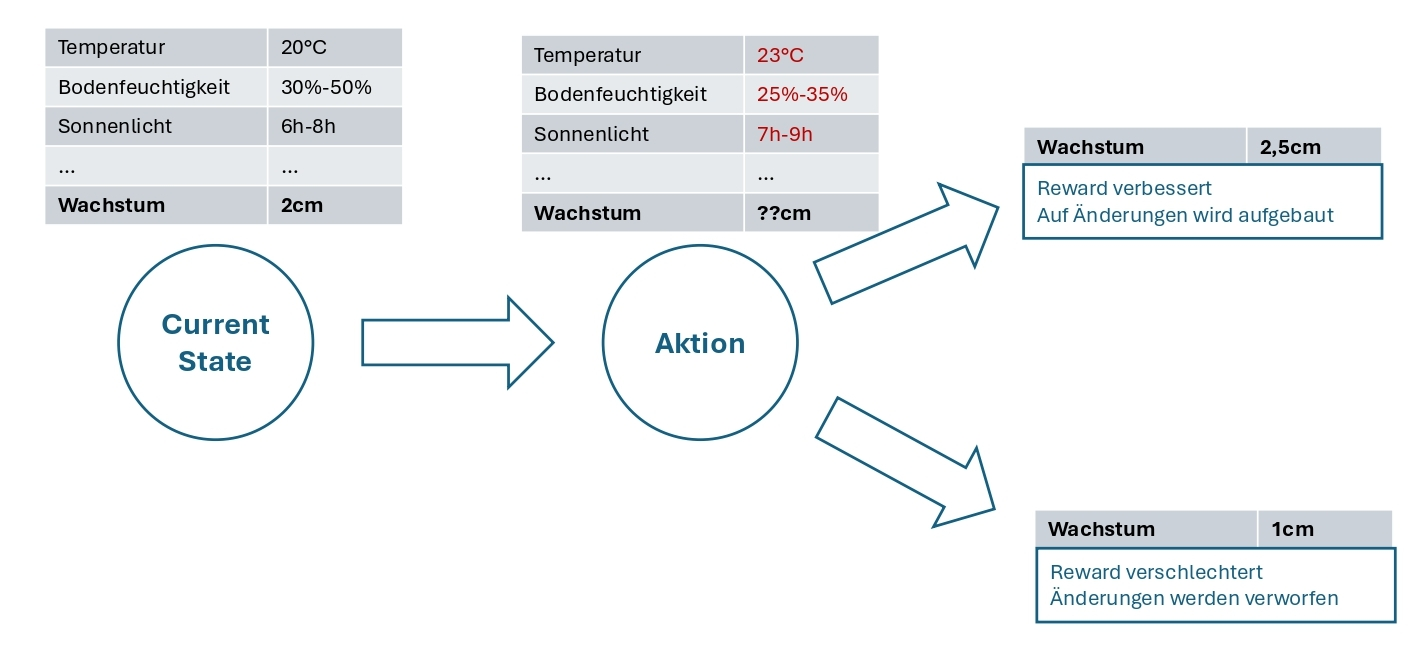
\includegraphics[width=\textwidth]{images/machineDiagram.jpg}
\caption{Genereller Workflow des Q-Learning Algorithmus}\cite{rainpoint_smart_timer}
\label{fig:rainpointDiagram}
\end{figure}

Die Python-Bibliothek Numpy erlaubt auf einfache Weise die Berechnungen für den Algorithmus. Hierbei werden die State-Werte der Umgebung zufällig verändert, der Reward (das Wachstum der Pflanze) bestätigt die getätigten Veränderungen oder widerlegt diese.\cite{mathworks2024qlearning} Eine Lern-Rate setzt fest wie stark es die Werte pro Iteration verändern darf. Dies ist von entscheidender Bedeutung für den Erfolg des Systems.

Nach genügend Iterationen mit der gleichen Pflanzengattung können so pro Pflanze verbesserte Umgebungsvariablen für die verschiedenen Wachstumsphasen bestimmt werden.
